\documentclass{article}
\usepackage{amssymb}
\usepackage{amsmath}
\usepackage{gensymb}
\usepackage{enumerate}
\usepackage{tikz}
\usetikzlibrary{positioning}
\usepackage[
nonumberlist, %do not show page numbers
nopostdot,    %do not add additional periods
acronym,      %generate acronym listing
toc,          %show listings as entries in table of contents
section]      %use section level for toc entries
{glossaries}
\usepackage[automake]{glossaries-extra}

\loadglsentries{glossary}
\makeglossaries

\newcommand{\printGls}[1]{%
    \textbf{\Gls{#1}} - \glsentrydesc{#1}%
}
\newcommand{\printGlspl}[1]{%
    \textbf{\Glspl{#1}} - \glsentrydesc{#1}%
}
\newcommand{\textiff}{\text{ iff }}

% PROOF SCRATCHWORK COMMANDS (Used to create Tikz givens/goals diagrams).
% Counter for automatic naming
\newcounter{proofboxnum}

\newcommand{\beginProofBoxes}[2]{
    % Initialize counter and first two boxes
    \setcounter{proofboxnum}{1}
    \node[draw, rectangle, text width=5cm, align=center] (given\theproofboxnum) {\textbf{Givens:}\\#1};
    \node[draw, rectangle, text width=5cm, align=center, right=0.5cm of given\theproofboxnum] (goal\theproofboxnum) {\textbf{Goals:}\\#2};
        
    % Increment the box number
    \stepcounter{proofboxnum}
}

\newcommand{\addProofBoxes}[2]{
    % Calculate previous box numbers
    \pgfmathtruncatemacro{\previousgiven}{\theproofboxnum - 1}
    \pgfmathtruncatemacro{\previousgoal}{\theproofboxnum - 1}
    
    % Add new boxes
    \node[draw, rectangle, text width=5cm, align=center, below=0.5cm of given\previousgiven] (given\theproofboxnum) {\textbf{Givens:}\\#1};
    \node[draw, rectangle, text width=5cm, align=center, right=0.5cm of given\theproofboxnum] (goal\theproofboxnum) {\textbf{Goals:}\\#2};
    
    % Draw arrows
    \draw[->] (given\previousgiven) -- (given\theproofboxnum);
    \draw[->] (goal\previousgoal) -- (goal\theproofboxnum);
     
    % Increment the box number
    \stepcounter{proofboxnum}
}

\usepackage{tikz}
\usetikzlibrary{positioning}

\title{Proofs}
\author{Axel Sorenson}
\date{July 11th, 2024}

\begin{document}
\maketitle

\section{Proof Strategies}
Mathematicians usually state the answer to a mathematical question in the form of a \gls{theorem}, such that if the assumptions stated within (which are called the \glspl{hypothesis}) are true, then some conclusion must also be true. Free variables within the theorem, if assigned specific values from the \gls{universe of discourse}, turns the theorem into an \gls{instance} of the theorem. For all instances of the theorem such that the hypotheses are true, the conclusion must also be true in order for the theorem to be correct. If even one instance has all true hypotheses and a false conclusion, then the theorem is incorrect. This is called a \gls{counterexample} to the theorem.\\

\noindent The following is a general structure of a proof:\\
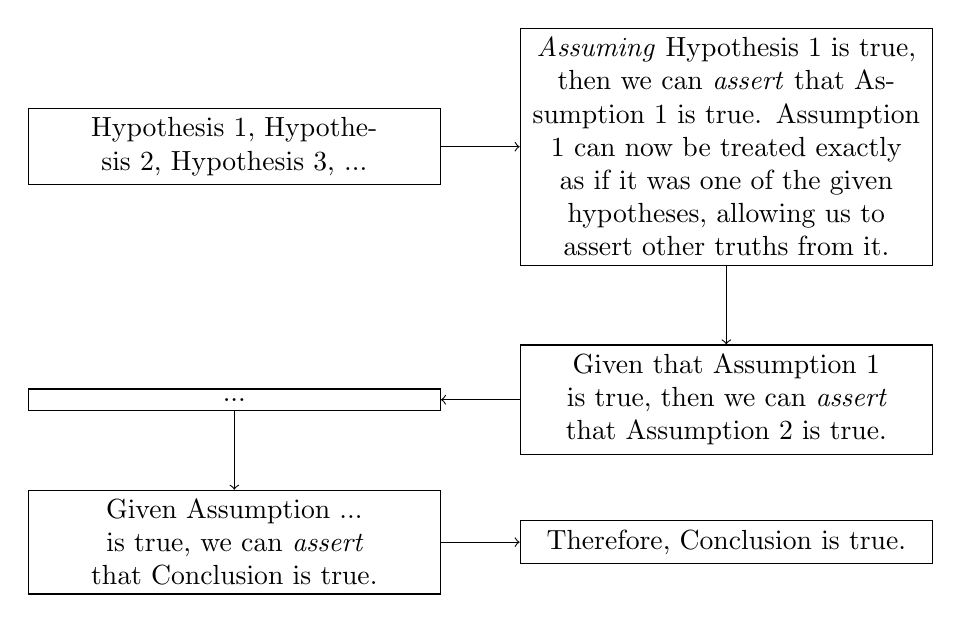
\begin{tikzpicture}[node distance=1cm, auto]
    % Define the boxes
    \node[draw, rectangle, text width=5cm, align=center] (box1) {Hypothesis 1, Hypothesis 2, Hypothesis 3, ...};
    \node[draw, rectangle, text width=5cm, align=center, right=of box1] (box2) {\textit{Assuming} Hypothesis 1 is true, then we can \textit{assert} that Assumption 1 is true. Assumption 1 can now be treated exactly as if it was one of the given hypotheses, allowing us to assert other truths from it.};
    \node[draw, rectangle, text width=5cm, align=center, below=of box2] (box3) {Given that Assumption 1 is true, then we can \textit{assert} that Assumption 2 is true.};
    \node[draw, rectangle, text width=5cm, align=center, left=of box3] (box4) {...};
    \node[draw, rectangle, text width=5cm, align=center, below=of box4] (box5) {Given Assumption ... is true, we can \textit{assert} that Conclusion is true.};
    \node[draw, rectangle, text width=5cm, align=center, right=of box5] (box6) {Therefore, Conclusion is true.};
    
    % Draw arrows between the boxes
    \draw[->] (box1) -- (box2);
    \draw[->] (box2) -- (box3);
    \draw[->] (box3) -- (box4);
    \draw[->] (box4) -- (box5);
    \draw[->] (box5) -- (box6);
\end{tikzpicture} \\
We can also transform proofs into equivalent proofs that are easier to write about, much like how we can transform equations (such as adding or subtracting values on both sides of an equation). So we can do a transformation of a simple proof like this:

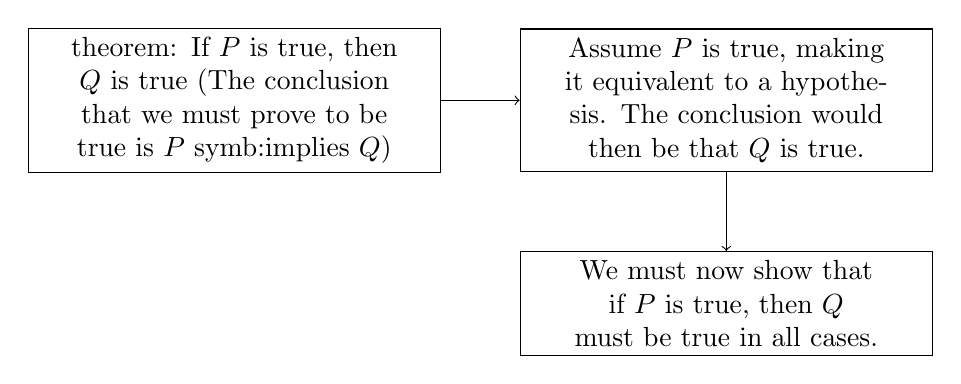
\begin{tikzpicture}[node distance=1cm, auto]
    \node[draw, rectangle, text width=5cm, align=center] (box1) {\Gls{theorem}: If $P$ is true, then $Q$ is true (The conclusion that we must prove to be true is $P \text{ \gls{symb:implies} } Q$)};
    \node[draw, rectangle, text width=5cm, align=center, right=of box1] (box2) {Assume $P$ is true, making it equivalent to a hypothesis. The conclusion would then be that $Q$ is true.};
    \node[draw, rectangle, text width=5cm, align=center, below=of box2] (box3) {We must now show that if $P$ is true, then $Q$ must be true in all cases.};
    
    \draw[->] (box1) -- (box2);
    \draw[->] (box2) -- (box3);
\end{tikzpicture} \\
This transformation essentially means that if our theorem we are trying to prove has the form $P \rightarrow Q$, then we can assume $P$ to be true, adding it to our list of hypotheses, and then change the conclusion from $P \rightarrow Q$ to $Q$. This new form of the proof might be easier to solve, depending on the complexity of what $P$ and $Q$ is. Note that this doesn't solve the proof - it is just a transformation that can be used to create a new (hopefully easier) problem that must be solved.\\

\noindent A proof may have several transformations applied to it over time, and it's important that we keep track of the results of this sequence of transformations. We therefore introduce the following terminology. We will refer to the statements that are known or assumed to be true at some point in the course of figuring out a proof as \glspl{given}, and the statement that remains to be proven at that point as the \gls{goal}. When you are starting to figure out a proof, the givens will be just the hypotheses of the theorem you are proving, but they may later include other statements that have been inferred from the hypotheses or added as new assumptions as the result of some transformation of the problem. The goal will initially be the conclusion of the theorem, but it may be changed several times in the course of figuring out a proof.\\

\noindent Note that the transformation technique described earlier is best described as enacted upon givens and goals as it can be used on transformations of the original proof rather than the proof itself. Here's an example of this transformation in action:

\noindent Suppose $a$ and $b$ are real numbers. Prove that if $0 < a < b$ then $a^2 < b^2$.\\
Transformation:\\
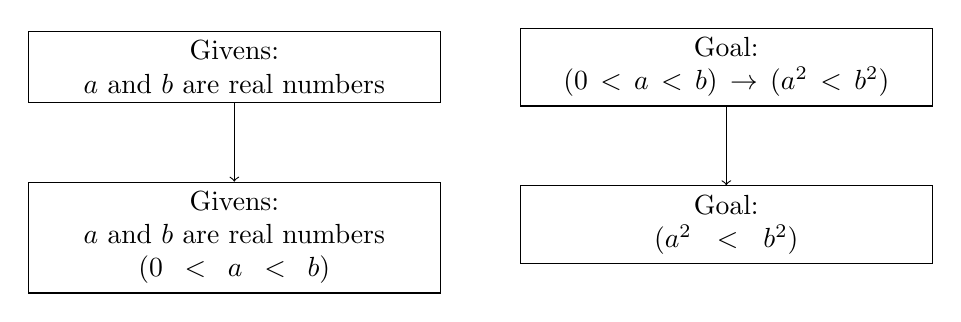
\begin{tikzpicture}[node distance=1cm, auto]
    \node[draw, rectangle, text width=5cm, align=center] (box1) {
        Givens:\\
        $a$ and $b$ are real numbers
    };
    \node[draw, rectangle, text width=5cm, align=center, right=of box1] (box2) {
        Goal:\\
        $(0 < a < b) \rightarrow (a^2 < b^2)$
    };

    \node[draw, rectangle, text width=5cm, align=center, below=of box1] (box3) {
        Givens:\\
        $a$ and $b$ are real numbers\\
        $(0 < a < b)$
    };
    
    \node[draw, rectangle, text width=5cm, align=center, below=of box2] (box4) {
        Goal:\\
        $(a^2 < b^2)$
    };

    \draw[->] (box1) -- (box3);
    \draw[->] (box2) -- (box4);
\end{tikzpicture} \\
Multiplying $a < b$ by $a$ gives us $a^2 < ab$ and multiplying $a < b$ by $b$ gives us $ab < b^2$. Together that makes $a^2 < ab < b^2$, making our goal, $a^2 < b^2$, true.

\clearpage
\printglossary[type=\acronymtype,style=long]  % list of acronyms
\printglossary[type=symbolslist,style=long]   % list of symbols
\printglossary[type=main]                     % main glossary
\end{document}
